    \documentclass[dvipsnames]{beamer}
    \usetheme{Madrid}
    \usefonttheme{professionalfonts}
    \usepackage{
        amsmath,
        amssymb,
        fouriernc, % fourier font w/ new century book
        fancyhdr, % page styling
        lastpage, % footer fanciness
        hyperref, % various links
        setspace, % line spacing
        amsthm, % newtheorem and proof environment
        mathtools, % \Aboxed for boxing inside aligns, among others
        float, % Allow [H] figure env alignment
        enumerate, % Allow custom enumerate numbering
        graphicx, % allow includegraphics with more filetypes
        wasysym, % \smiley!
        upgreek, % \upmu for \mum macro
        listings, % writing TrueType fonts and including code prettily
        tikz, % drawing things
        booktabs, % \bottomrule instead of hline apparently
        cancel % can cancel things out!
    }
    \usepackage[
        labelfont=bf, % caption names are labeled in bold
        font=scriptsize % smaller font for captions
    ]{caption}
    \usepackage[font=scriptsize]{subcaption} % subfigures

    \newcommand*{\scinot}[2]{#1\times10^{#2}}
    \newcommand*{\bra}[1]{\left<#1\right|}
    \newcommand*{\ket}[1]{\left|#1\right>}
    \newcommand*{\dotp}[2]{\left<#1\,\middle|\,#2\right>}
    \newcommand*{\rd}[2]{\frac{\mathrm{d}#1}{\mathrm{d}#2}}
    \newcommand*{\pd}[2]{\frac{\partial#1}{\partial#2}}
    \newcommand*{\rtd}[2]{\frac{\mathrm{d}^2#1}{\mathrm{d}#2^2}}
    \newcommand*{\ptd}[2]{\frac{\partial^2 #1}{\partial#2^2}}
    \newcommand*{\md}[2]{\frac{\mathrm{D}#1}{\mathrm{D}#2}}
    \newcommand*{\norm}[1]{\left|\left|#1\right|\right|}
    \newcommand*{\abs}[1]{\left|#1\right|}
    \newcommand*{\pvec}[1]{\vec{#1}^{\,\prime}}
    \newcommand*{\svec}[1]{\vec{#1}\;\!}
    \newcommand*{\bm}[1]{\boldsymbol{\mathbf{#1}}}
    \newcommand*{\expvalue}[1]{\left<#1\right>}
    \newcommand*{\ang}[0]{\text{\AA}}
    \newcommand*{\mum}[0]{\upmu \mathrm{m}}
    \newcommand*{\at}[1]{\left.#1\right|}

    \let\Re\undefined
    \let\Im\undefined
    \DeclareMathOperator{\Res}{Res}
    \DeclareMathOperator{\Re}{Re}
    \DeclareMathOperator{\Im}{Im}
    \DeclareMathOperator{\Log}{Log}
    \DeclareMathOperator{\Arg}{Arg}
    \DeclareMathOperator{\Tr}{Tr}
    \DeclareMathOperator{\E}{E}
    \DeclareMathOperator{\Var}{Var}
    \DeclareMathOperator*{\argmin}{argmin}
    \DeclareMathOperator*{\argmax}{argmax}
    \DeclareMathOperator{\sgn}{sgn}
    \DeclareMathOperator{\diag}{diag\;}

    \DeclarePairedDelimiter\p{\lparen}{\rparen}
    \DeclarePairedDelimiter\s{\lbrack}{\rbrack}
    \DeclarePairedDelimiter\z{\lbrace}{\rbrace}

    % \everymath{\displaystyle} % biggify limits of inline sums and integrals
    \tikzstyle{circ} % usage: \node[circ, placement] (label) {text};
        = [draw, circle, fill=white, node distance=3cm, minimum height=2em]
    \definecolor{commentgreen}{rgb}{0,0.6,0}
    \lstset{
        basicstyle=\ttfamily\footnotesize,
        frame=single,
        numbers=left,
        showstringspaces=false,
        keywordstyle=\color{blue},
        stringstyle=\color{purple},
        commentstyle=\color{commentgreen},
        morecomment=[l][\color{magenta}]{\#}
    }

\begin{document}

\pagestyle{fancy}
\rfoot{Yubo Su}
\cfoot{\thepage/\pageref{LastPage}}

\title[Exciting Internal Gravity Waves]{Exciting Internal Gravity Waves, Toy
Problem}
\subtitle[]{Mar 23, 2018 Group Meeting}
\author[Yubo Su]{Yubo Su}
\date{Mar 23, 2018}

\frame{\titlepage}

\begin{frame}
    \frametitle{Problem Setup}
    \framesubtitle{Problem Statement}
    \begin{itemize}
        \item Eventual objective: simulate IGW breaking in WDs, compute
            energy/angular momentum dissipation profiles.
        \item Toy problem: 2D hydrodynamics with driving boundary condition.
        \item Begin with linear incompressible case, equations:
        \begin{subequations}\label{se:eom}
            \begin{align}
                \pd{\rho_1}{t} &= 0,\\
                \vec{\nabla} \cdot \vec{u}_1 &= 0,\\
                \pd{\vec{u}_1}{t} &= -\frac{\vec{\nabla}P_1}{\rho_0} + \vec{g}.
            \end{align}
        \end{subequations}

        \item Consider stratified atmosphere $\rho_0(x, z, t) = \rho_0
            e^{-z/H}$.
    \end{itemize}
\end{frame}

\begin{frame}
    \frametitle{Problem Setup}
    \framesubtitle{Boundary Conditions}

    \begin{itemize}
        \item Four variables ($\rho_1, P_1, u_{1x}, u_{1z}$), all first order in
            equations of motion, four boundary conditions.

        \item Periodic BCs in $x$ (2).

        \item Wavelike solutions $u_{1z} \propto e^{z/2H}e^{i\p*{k_xx + k_zz -
            \omega t}}$, $u_{1x}, P_1, \rho_1$ similar up to phase and terms
            $\sim \mathcal{O}\p*{H^{-1}} \ll k_z$.

        \item Obeys dispersion relation
            \begin{equation}
                \omega^2 = \frac{N^2k_x^2}{k_x^2 + k_z^2 + \frac{1}{4H^2}}.
            \end{equation}

        \item Driven bottom BC\@: $u_{1z}(x, 0, t) = A\cos \p*{k_xx + \omega t}$
            (1).
    \end{itemize}
\end{frame}

\begin{frame}
    \frametitle{Problem Setup}
    \framesubtitle{Top Boundary Condition}

    \begin{itemize}
        \item Top BC can be chosen Dirichlet $u_{1z}(x, L_z, t) = 0$,
            analytically tractable as linear combination of $\pm k_z$ solutions.

        \item Driving term will pump energy into the system, without dissipation
            becomes like driven undamped SHO\@. In full nonlinear problem not an
            issue\dots

        \item More realistically, two solutions: radiative boundary conditions
            and damping zone.

        \item We use damping zone, add term $\pd{}{t}\vec{q} = L\vec{q}
            - f(z)\p*{\vec{q} - \vec{q}_0}$ where
            \begin{equation}
                f(z) =
                \begin{cases}
                    \Gamma \s*{
                        1 - \frac{\p*{z - L_z}^2}
                            {\p*{z_{damp} - L_z}^2}
                    }
                        & z > z_{damp}\\
                    0 & z < z_{damp}
                \end{cases}.
            \end{equation}
    \end{itemize}
\end{frame}

\begin{frame}
    \frametitle{Results}
    \framesubtitle{Problem Statement Summary}

    \begin{itemize}
        \item Linear incompressible 2D hydrodynamics with periodic BCs in $x$,
            driving term at $z = 0$ and either Dirichlet or reflection-free BCs
            at $z = L_z$.

        \item Spectral code Dedalus, exponential convergence for shock-free
            hydrodynamics.
    \end{itemize}
\end{frame}

\begin{frame}
    \frametitle{Results}
    \framesubtitle{Waveform Agreement}

    \begin{figure}[!h]
        \centering
        \begin{subfigure}{0.37\textwidth}
            \centering
            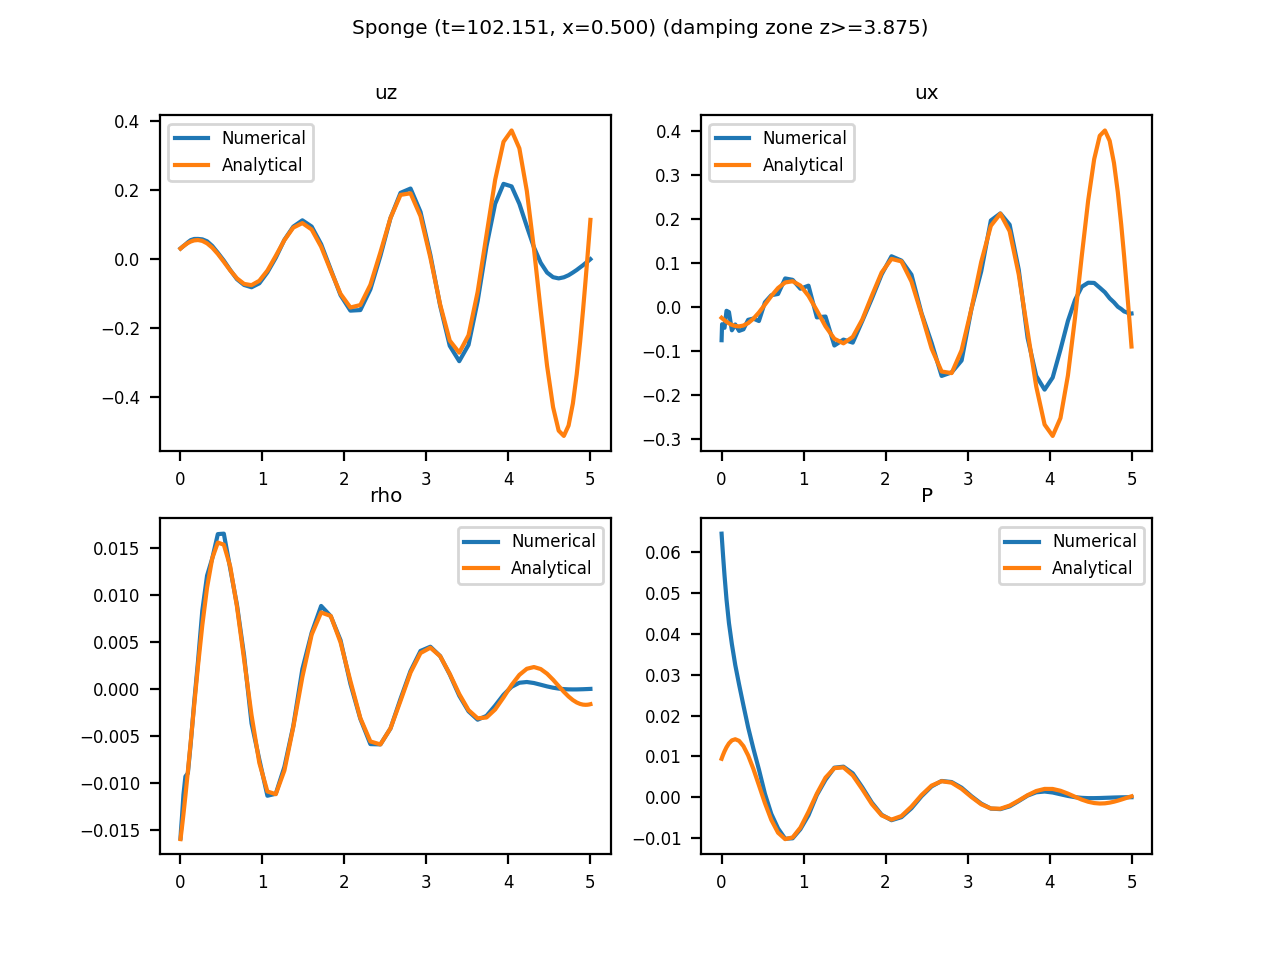
\includegraphics[width=\textwidth]{../sims/2d_strat/agree_plots/sponge_0.png}
        \end{subfigure}
        \begin{subfigure}{0.37\textwidth}
            \centering
            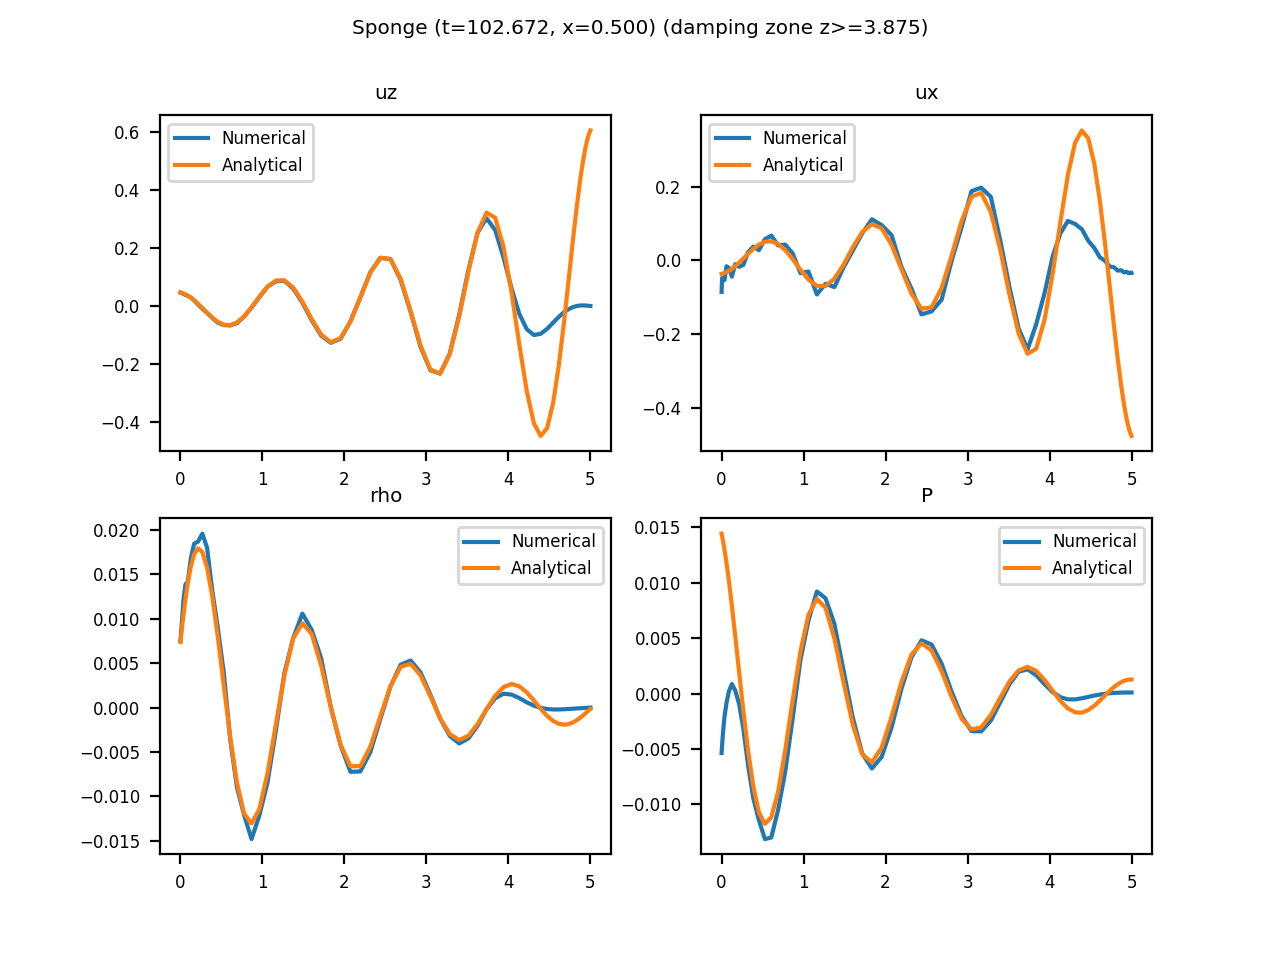
\includegraphics[width=\textwidth]{../sims/2d_strat/agree_plots/sponge_1.png}
        \end{subfigure}

        \begin{subfigure}{0.37\textwidth}
            \centering
            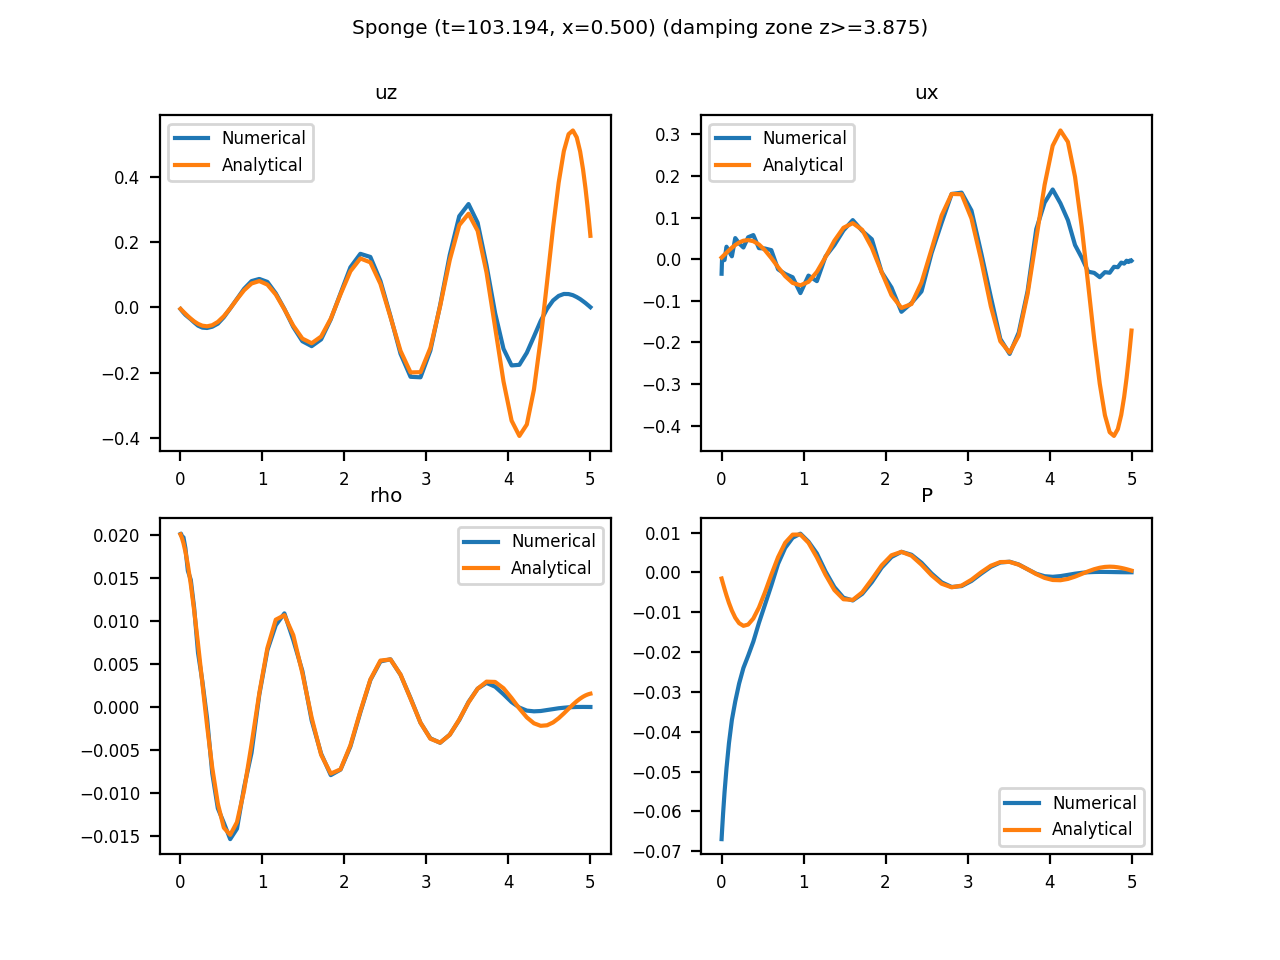
\includegraphics[width=\textwidth]{../sims/2d_strat/agree_plots/sponge_2.png}
        \end{subfigure}
        \begin{subfigure}{0.37\textwidth}
            \centering
            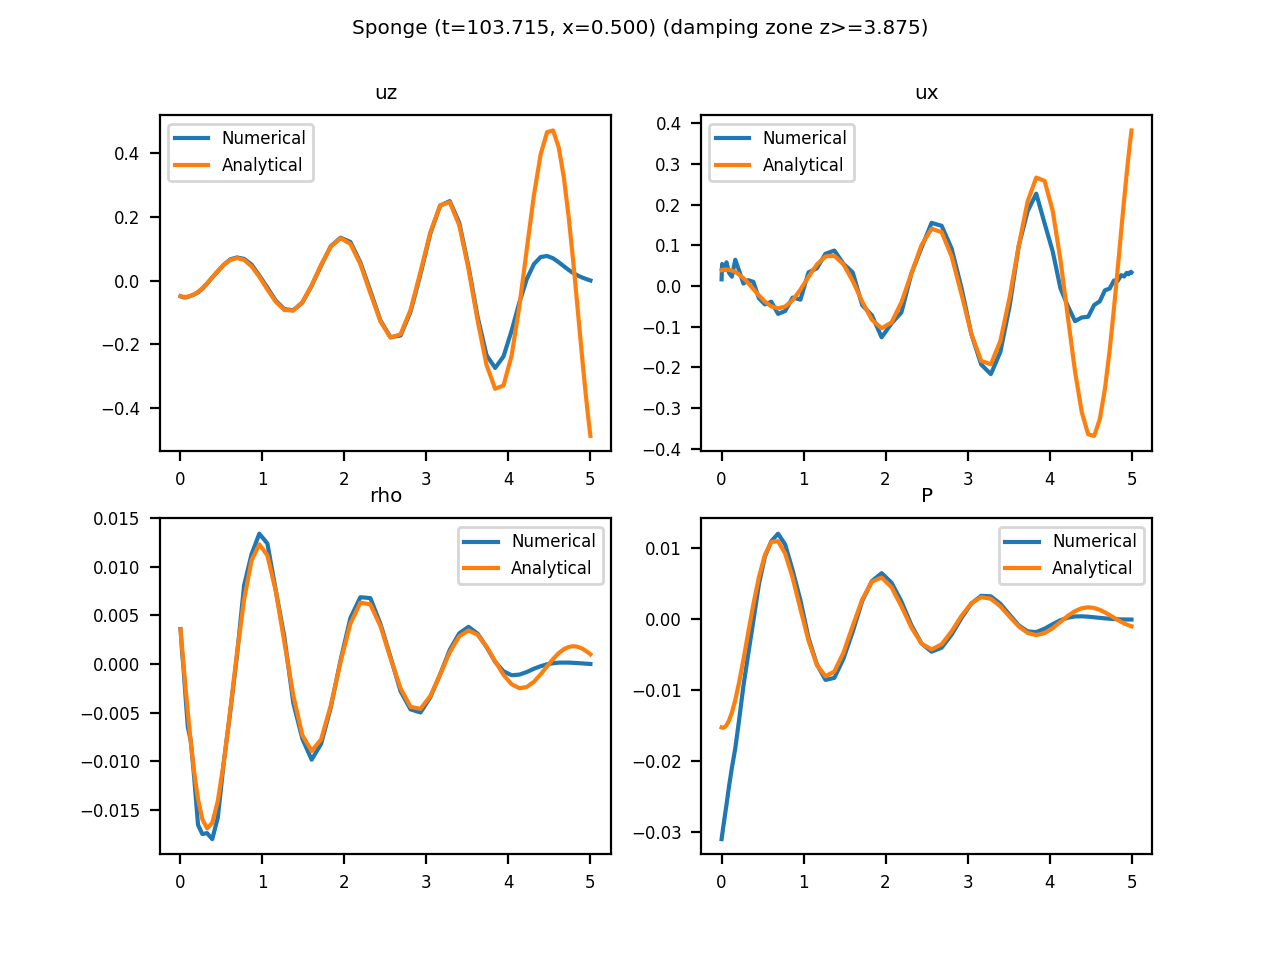
\includegraphics[width=\textwidth]{../sims/2d_strat/agree_plots/sponge_3.png}
        \end{subfigure}
        \caption{Numerical and analytical solutions agree. Numerics chooses
        $v_{gz} > 0$.}\label{fig:sponge_agree}
    \end{figure}
\end{frame}

\begin{frame}
    \frametitle{Results}
    \framesubtitle{Convergence Tests}

    \begin{itemize}
        \item $RMS_i = \frac{\sqrt{\sum\limits_{x, z, t} \p*{u_{1z}^{(i)}(x, z,
            t) - u_{1z}^{(N)}(x, z, t)}^2}}{\sqrt{ \sum\limits_{x, z, t}
            \p*{u_{1z}^{(N)}(x, z, t)}^2}}$
    \end{itemize}
    \begin{figure}[!h]
        \centering
        \begin{subfigure}{0.37\textwidth}
            \centering
            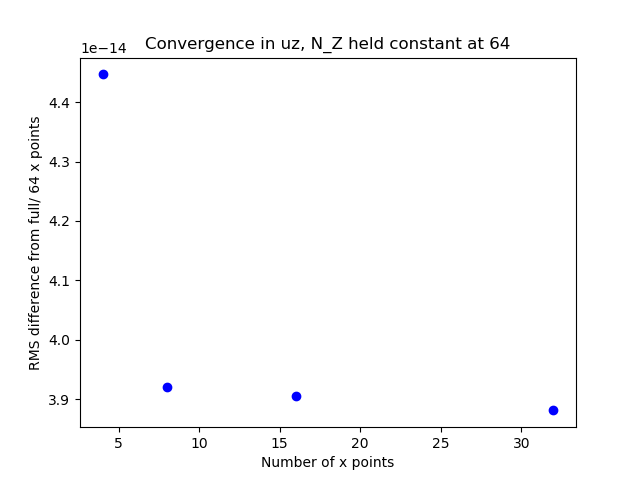
\includegraphics[width=\textwidth]{../sims/2d_strat_conv/x_conv.png}
        \end{subfigure}
        \begin{subfigure}{0.37\textwidth}
            \centering
            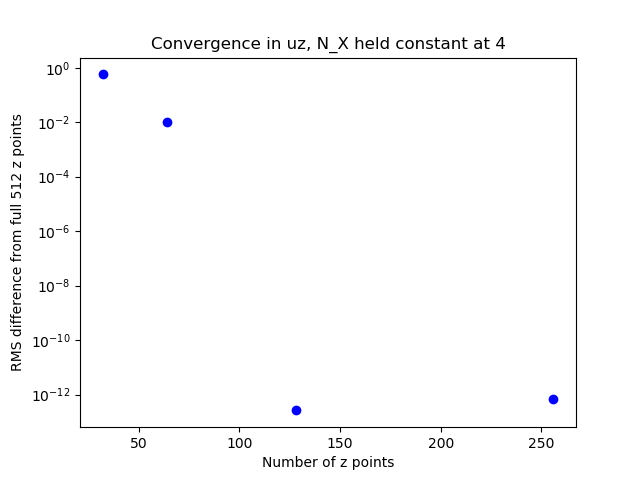
\includegraphics[width=\textwidth]{../sims/2d_strat_conv/z_conv.png}
        \end{subfigure}
        \caption{Convergences of RMS over grid resolution. Note the exponential
        convergence in $z$ to machine precision (since $x$ is always
        monochromatic, increasing resolution does little).}\label{fig:convsv}
    \end{figure}
\end{frame}

\begin{frame}
    \frametitle{Future Work}
    \framesubtitle{Future Work}

    \begin{itemize}
        \item Nonlinear 2D incompressible hydro; does it reproduce the above
            results in the small-perturbation limit?

        \item Radiative boundary conditions?
    \end{itemize}
\end{frame}

\end{document}

